\section{Who's involved?}
%"I have nothing to hide, who cares about my personal data?"
\begin{frame}
	\frametitle{But...who cares?}
	\begin{center}
	\huge{"I have nothing to hide, who cares about my personal data?"}
	\end{center}

\end{frame}

\subsection{Surveillance} 
%I would start with the big picture of the Utah Datacenter
%NSA, snowden leaks
\begin{frame}
	\frametitle{Surveillance}
	\begin{itemize}
		\item Some intelligence organizations obviously do
		anti-terrorist researches and checks (and that's good!).
		\item Some intelligence organizations do that in wrong ways, a
		normal guy searched "Pressure cooking" and "knap sack" on google and
		FBI knocked at his house.
	\end{itemize}

	\begin{figure}
	\centering
		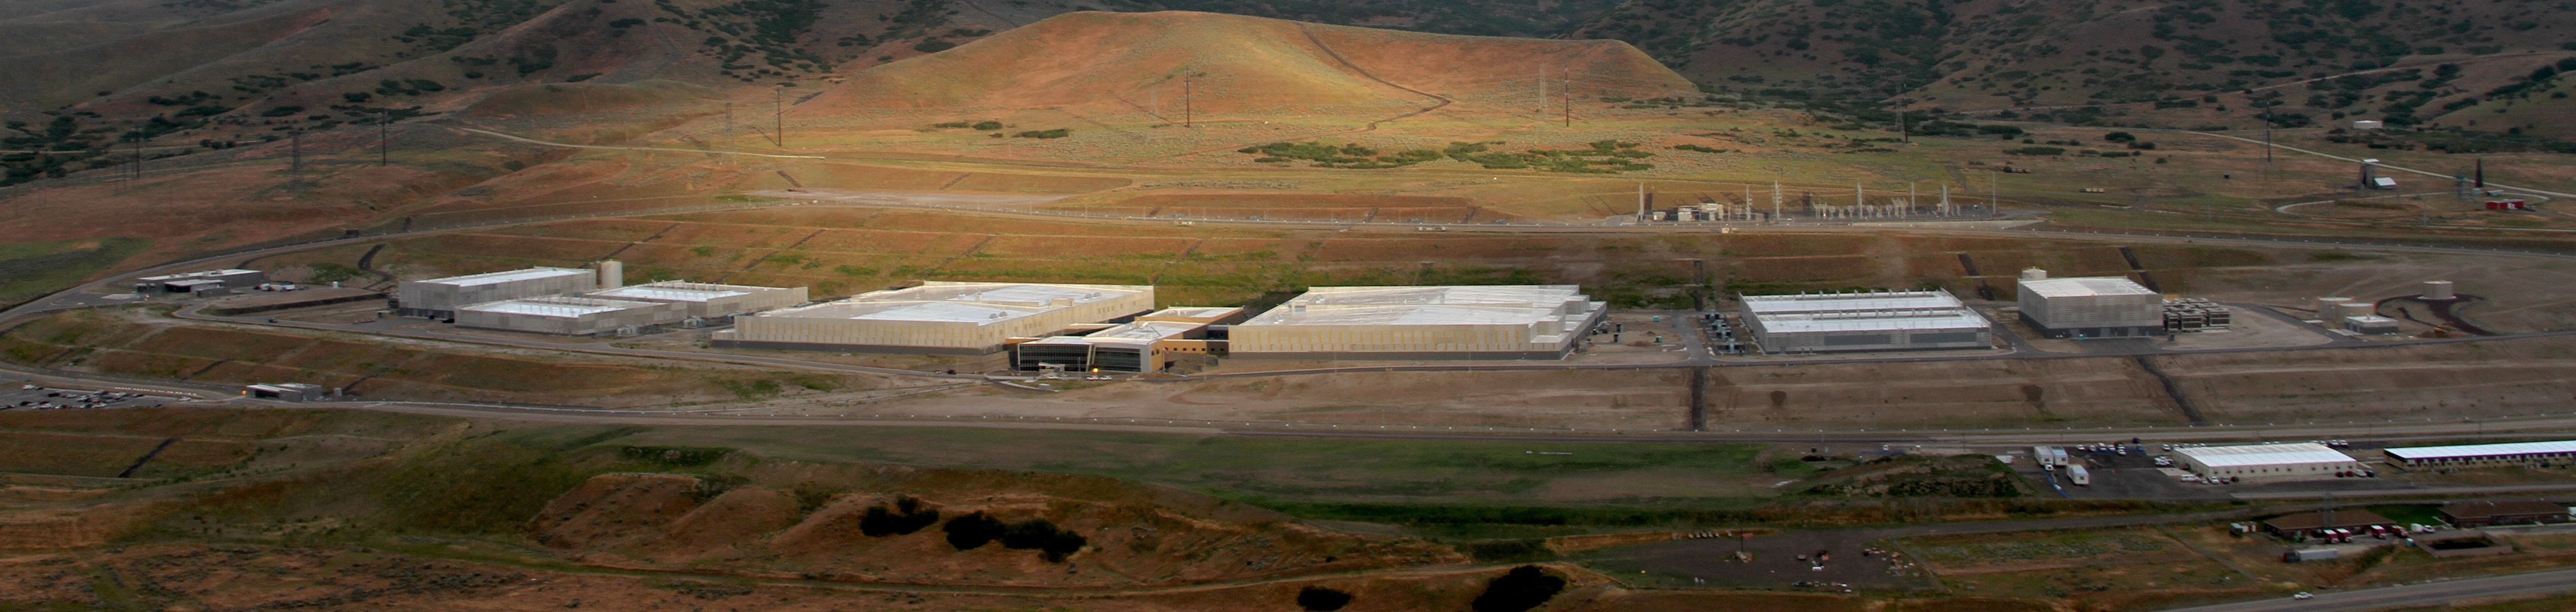
\includegraphics[scale=0.05]{imgs/utah}
		\caption{the utah NSA data
		center "Massive Data Repository", 90k-140k $m^2$}
	\end{figure}
\end{frame}

\begin{frame}
	\frametitle{NSA related projects}
	According to \textbf{Edward Snowden} leaks, the NSA organization has a
	lot of obscure and top secret projects:
	\begin{itemize}
		\item PRISM - Software to collect information about every internet communication (US)
		\begin{itemize}
			\item Related to some major companies.
		\end{itemize}
		\item Tempora - British Intelligence auditing software for
			internet and phone communications.
		\item MonsterMind - \textbf{Automated} reaction to attacks.
	\end{itemize}
		\hfill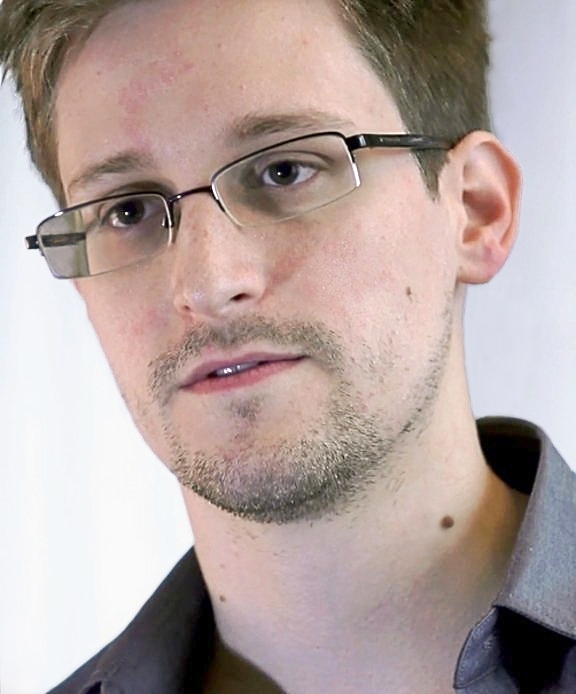
\includegraphics[scale=0.1]{imgs/snowden}
\end{frame}

\begin{frame}
	\frametitle{Other stories}
	\begin{itemize}
		\item PGP - "munitions export without a license".
		\item Lavabit - Request to give the public key of the site to
		the NSA.
		\item IP-sec - Snowden leaks revealed that NSA breaked (in
		collaboration with NIST?) the IP-sec suite and his encryption
		algorithms.
		\item Truecrypt - US intelligence failed to decrypt some disks
		encrypted with truecrypt and fifth amendment protected a suspect.
	\end{itemize}
\end{frame}

\begin{frame}
	\frametitle{Let's talk about numbers...}
	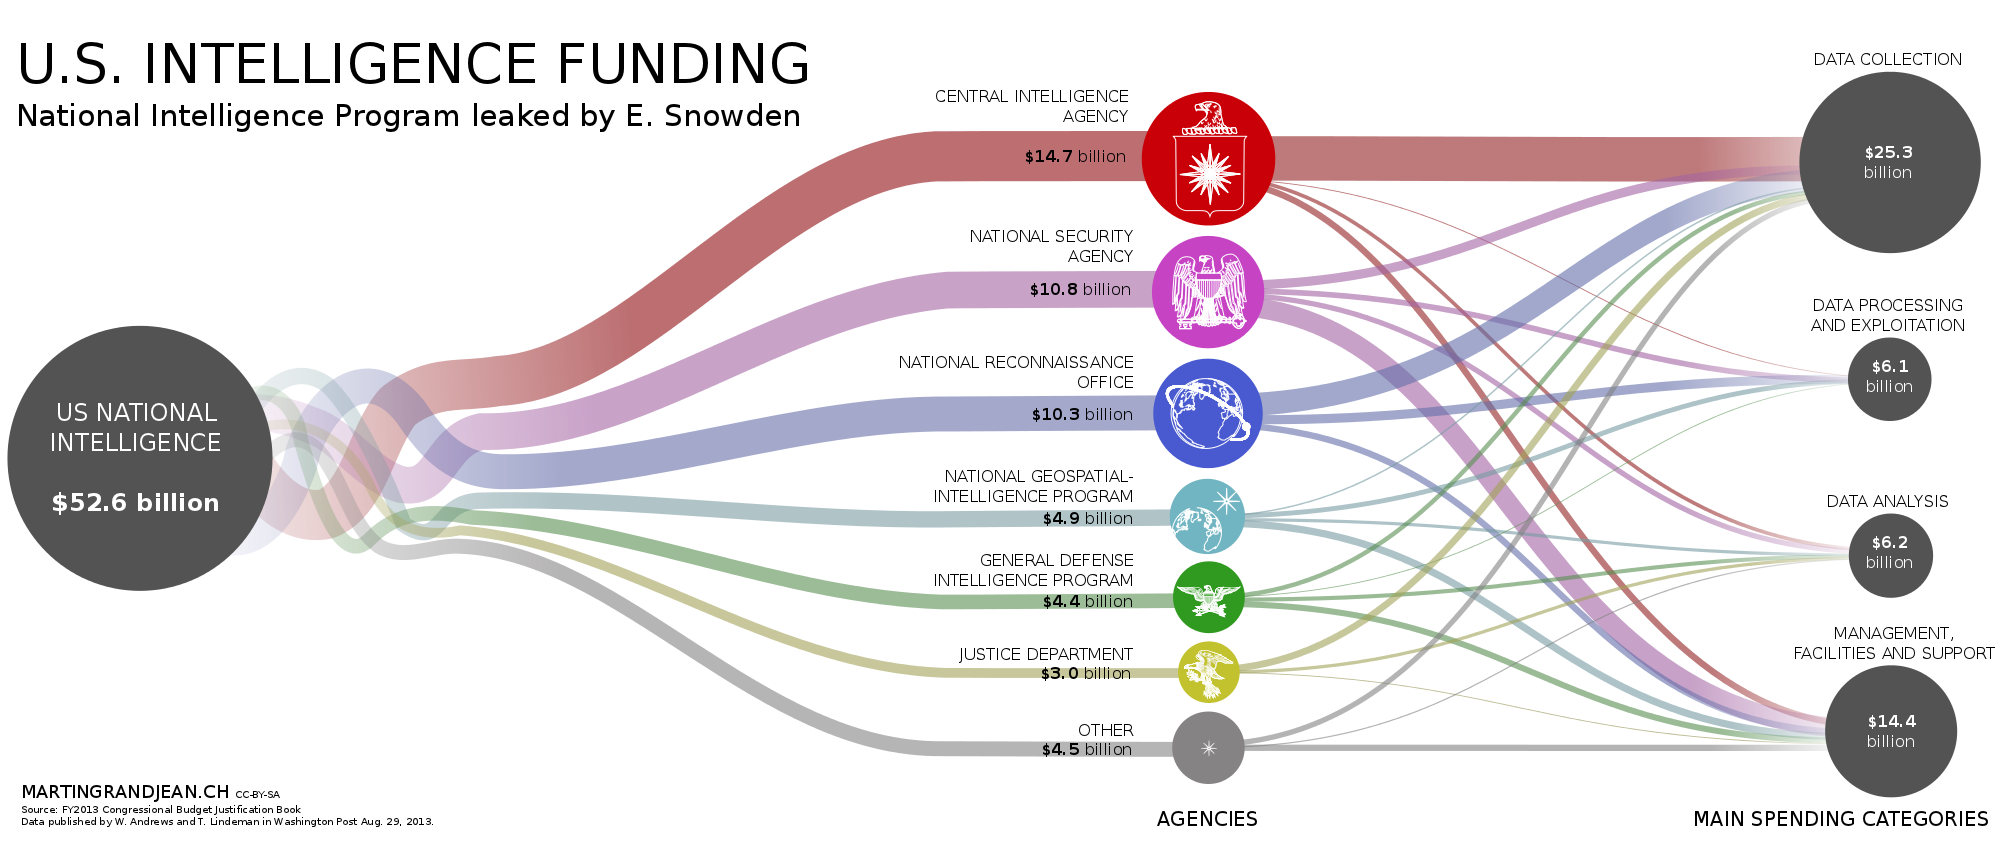
\includegraphics[width=\textwidth]{imgs/US_intelligence_budget}
\end{frame}

\begin{frame}
	\frametitle{...and leaks!}
	\begin{center}
		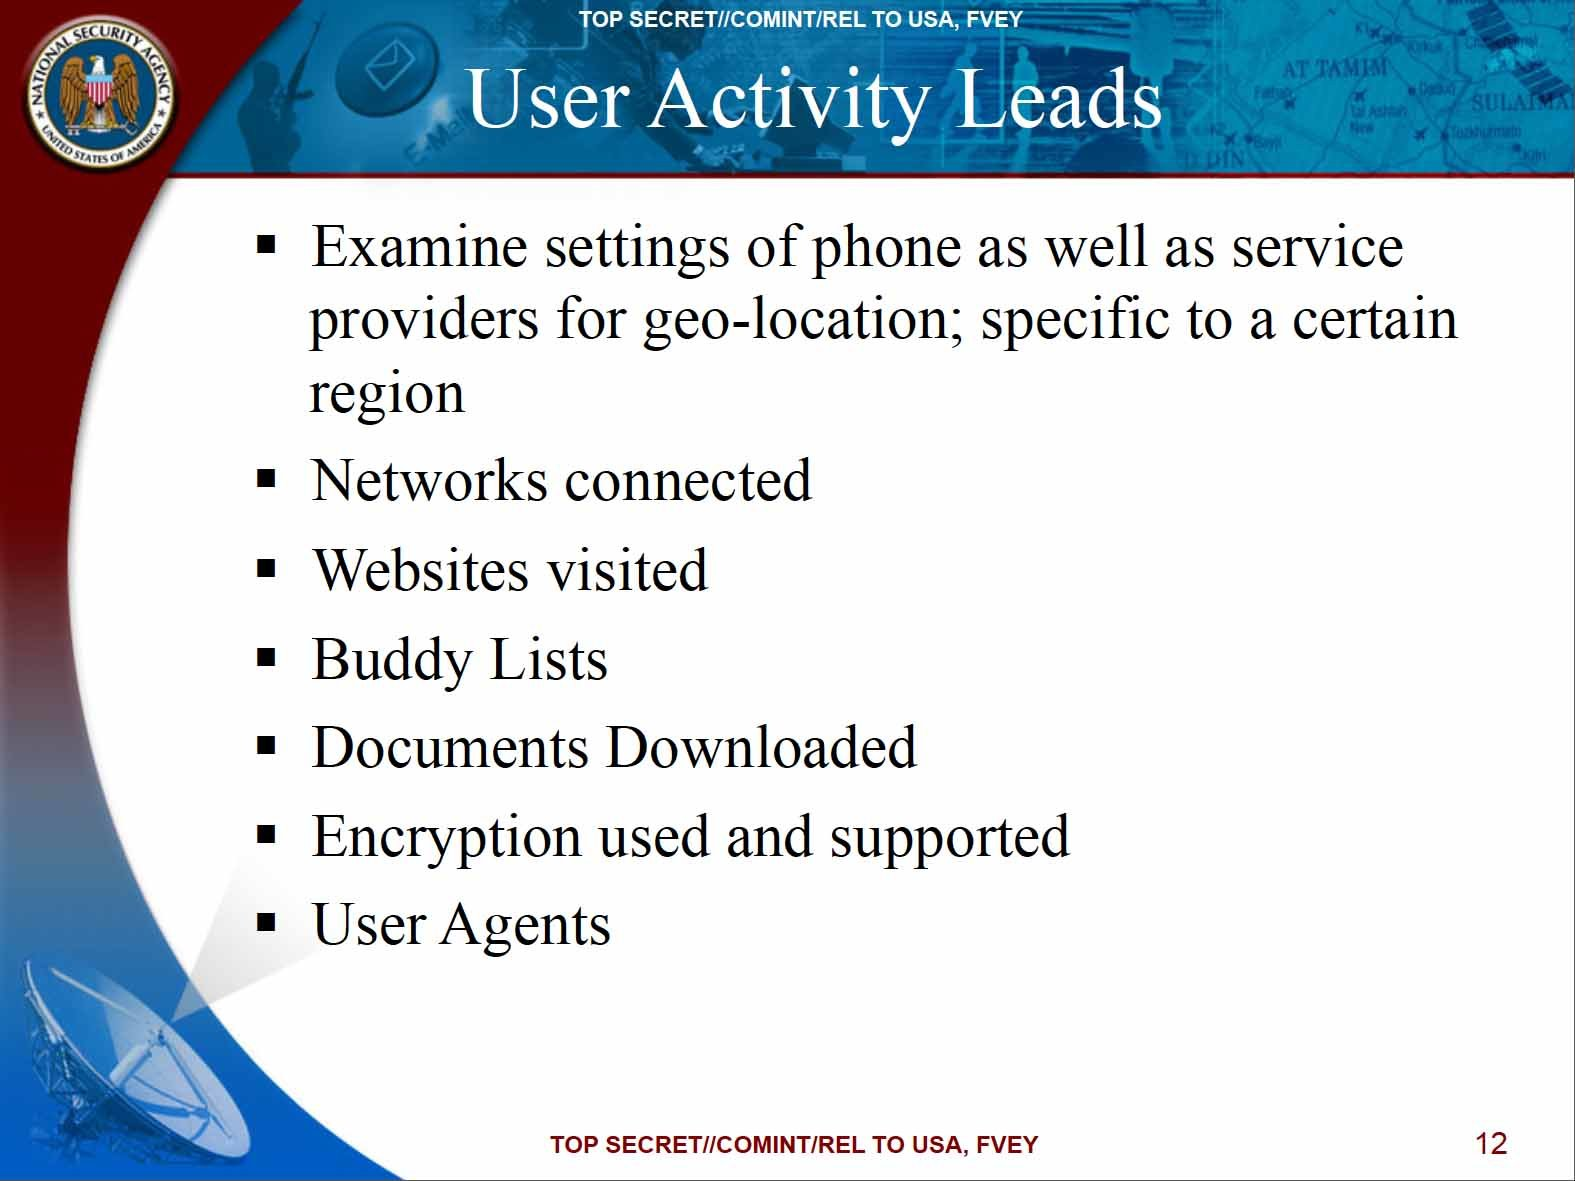
\includegraphics[scale=0.15]{imgs/nsa_leads}
	\end{center}
\end{frame}

\subsection{Obscuring}
\begin{frame}
	\frametitle{GEO-Obscuration}

	\tiny{Some places are sensitive to geo-obscuration (expecially
	east places like china or japan).}\\
	\begin{center}
	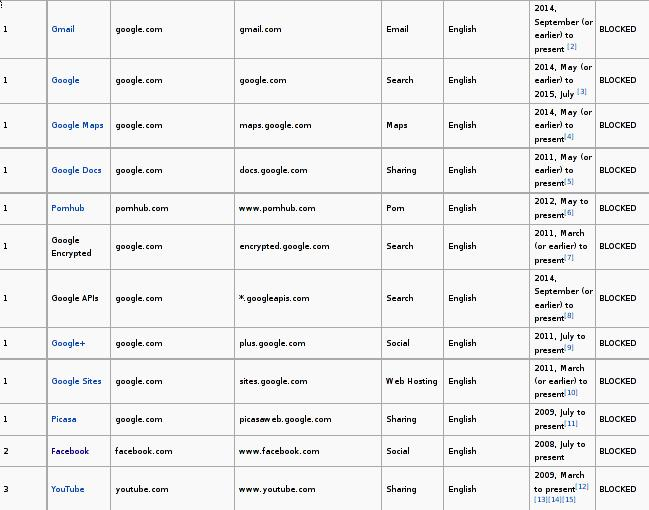
\includegraphics[scale=0.3]{imgs/blocked_china}
	\end{center}
\end{frame}

\begin{frame}
	\frametitle{SOPA and PIPA}
	\begin{itemize}
		\item Stop Online Piracy Act
		\item Gives the control of the obscuration of a site to the
		proprietary of the copyright (!) and to the government (!!!).
		\item In other words...everyone could obscure every site, that
		use copyrighted contents, from every search engine!
		\item Legal penalities and fees to the source of the publication.
		\item Incompatible with DMCA, GPL, etc...
		\item \textbf{Incompatible with VPN, ORs, proxies, etc (!!!).}
	\end{itemize}
\end{frame}

\subsection{Companies}
\begin{frame}
	\frametitle{Focused ADv}
	\begin{itemize}
		\item Some companies can do some users profilation.
		\item What you've searched, what you say or what you do can be a
		gold information on who you are and what you're going to do.
		\item Maybe the company inform you, and you have nothing to
		hide, but, you really want to say to a company sensible data?
		\item Imagine if a data leakage occurs and someone learns about
		your google searches...
		\item Coff, Coff, Windows 10 keylogger...
	\end{itemize}
\end{frame}

\subsection{Bad Guys}
%(identity stealing, money stealing, etc.)
\begin{frame}
	\frametitle{Not only powerful adversaries}
	\begin{itemize}
		\item Obviously the companies are not the only person interested
		in our real identity, someone could gain my IP, and/or my
		geolocation to break into my
		house when I'm out.
		\item So we must ensure our anonymity, just to have a form of
		security in addition to the classical ones.
		\item On the other hand, there is the identity stealing.
	\end{itemize}
\end{frame}
